\section{Abstraction Blocks: Thinking with Boxes}

\subsection{Formative Interviews: How Do Experts Collaborate?}
To investigate the role of abstraction in how experts communicate during collaboration, we observed three proficient illustrators recruited from a local drawing and illustration club perform a collaborative drawing task. In this task, the group made a single drawing together based on an open-ended prompt, ``Draw a scene of a place that makes you happy.'' We provided the group with paper, sticky notes, pencils, colored pens and markers, and a single large sheet of paper as the canvas for their drawing. We observed that experts used abstraction in three main ways.

First, experts used abstraction to quickly capture ideas from members of the group. In planning their drawing, the group first created several small thumbnail sketches on sticky notes as members generated ideas for various drawing compositions as part of their planning process (Figure \ref{fig:expert}). Creating small, abstract drawings is a common technique for visually generating ideas and solving problems \cite{poore1967composition,Poore1967}. In this collaborative context, this technique additionally functioned as a way to communicate and confirm thoughts between members of the group, throwing out various ``what if'' scenarios: \textit{``What if we made like ice cream dogs? I know that's silly, but it conveys happy.''} Sometimes a participant would sketch a thumbnail themselves and place it in the center to show the group their idea. Other times, a participant would draw a thumbnail sketch as a different participant was verbally describing their idea, while asking for confirmation that their sketch of the idea was accurate. In a post-interview, the experts mentioned that they learned the thumbnailing technique from their art education and practice.

\begin{figure}
\centering
  %\vspace{-0.2in}
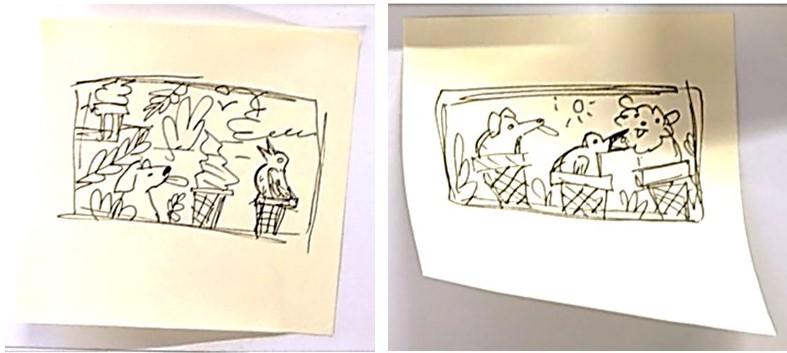
\includegraphics[width=\textwidth]{abstraction/figures/thumbnails.jpg}
\vspace{-0.2in}
  \caption{An expert participant sketched these two thumbnails to illustrate and explore alternate compositions for similar elements.}
  ~\label{fig:thumbnail}
  \vspace{-0.2in}
\end{figure}

Second, experts used abstraction to reduce unnecessary work by reusing elements that had already been drawn. For example, Figure \ref{fig:thumbnail} shows two thumbnail sketches that contain similar elements in different layouts and compositions. To choose a direction for their sketch, the group placed the thumbnail sketches in front of them and discussed to come to a consensus. These sketches conveyed relative positioning of sketch elements rather than specific details of the drawing. The group decided on an overall composition while adding in ideas contributed through other group members' thumbnails.

Lastly, experts used abstraction as a way to anchor discussions about how to proceed.
After deciding on an overall composition, the expert group  assigned work to each of its members. However, rather than assigning work based on areas of the canvas paper, the group delegated work based on the elements in the composition they had developed together: ``\textit{You draw the background since it's your design, you draw the foliage, and I'll draw the [character]?}'' This gave a clear sense in who would draw which part of the sketch and drew from their rough composition plan. 

% \begin{figure}
% \centering
%   %\vspace{-0.2in}
% 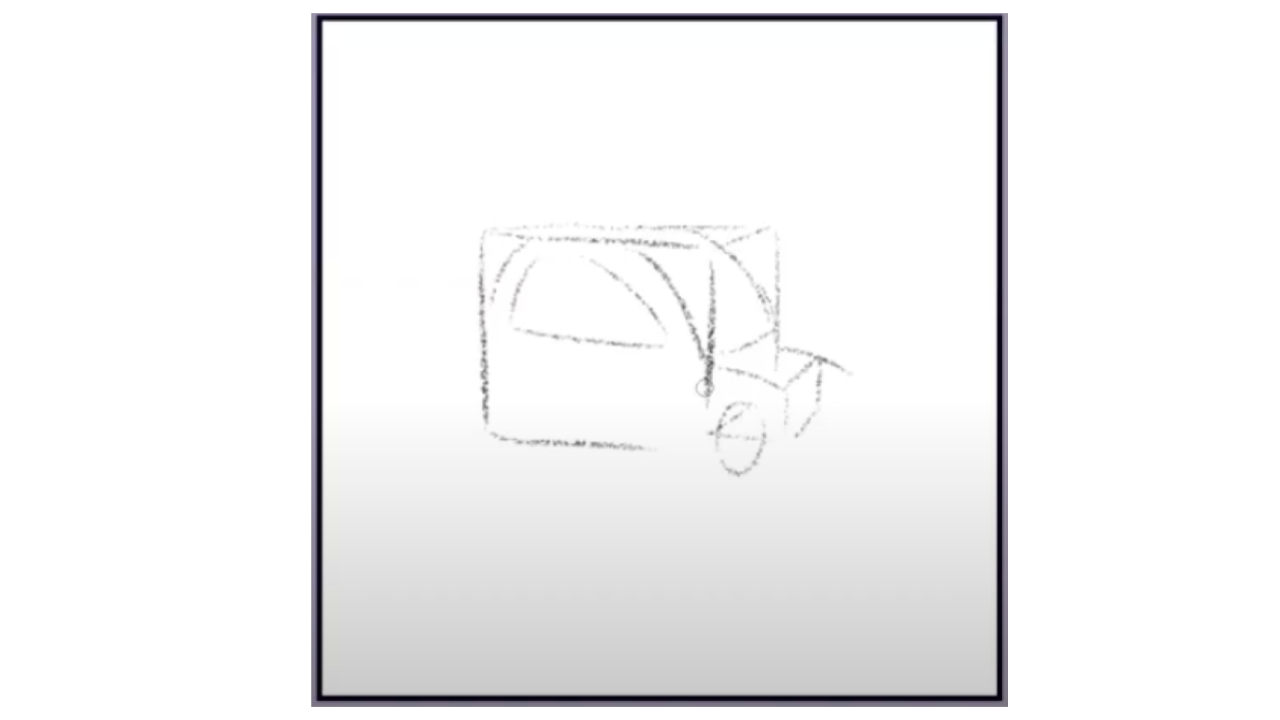
\includegraphics[width=.8\textwidth]{abstraction/figures/expertbox.png}
% \vspace{-0.2in}
%   \caption{An expert demonstrating how box shapes can be used as the basis for drawing nearly any object.}
%   ~\label{fig:expertbox}
%   \vspace{-0.2in}
% \end{figure}

After completing their rough sketch, the experts began adding details. This part of drawing process was much more improvisational; for example, individual members of the group freely colored in areas of the sketch with little or no coordination with other members of the group. In a post-interview, experts noted that the drawing phases did not require as much communication or coordination, since much of the sketch had been previously outlined, reflecting the key concepts of loosely coupled work and maintaining common ground \cite{olson2000distance}.

\subsection{Abstraction Blocks: Making the Abstract Concrete}
From prior work on expert abstraction strategies and our observations of the expert illustrators, we distill these strategies into \textit{abstraction blocks}. We implement these blocks using paper sticky notes as representations of blocking, or chunking, elements that can be shaped, edited, and moved around as desired (Figure \ref{fig:blocks}). We chose to characterize abstraction as abstraction blocks because we expected it would be easy for novices to understand and because it mimics common abstraction strategies used by experts in our chosen domain of drawing \cite{poore1967composition}. While sketches are an abstract representation themselves, novices especially still focus on details rather than exploratory goals during sketching \cite{welch2000sketching}. Encouraging participants to use blocks allows participants to convey rough composition without the need for sketching, emphasizes the spatial relationships between components of a drawing rather than its details, and express a creative vision without worrying about drawing skill or matching the aesthetic style of other collaborators.

